\chapter{ Технологический раздел}
\label{cha:technological}

    В данном разделе будут выбраны средства реализации ПО и представлен листинг кода. 

    \section{Средства реализации}
В качестве языка программирования для реализации программы был выбран язык C++ и фреймворк Qt, потому что:
\begin{itemize}
	\item язык C++ имеет высокую вычислительную производительность;
	\item язык C++ поддерживает различные стили программирования;
	\item в Qt существует удобный инструмент для тестирования - QtTest - который позволяет собирать тесты в группы, собирать результаты выполнения тестов, а также уменьшить дублирование кода при схожих объектах тестирования.
\end{itemize}

Для замеров времени использовался методы restart() и elapsed() класса QTime. Метод elapsed() возвращает количество миллисекунд, прошедших с момента последнего вызова start() или restart().

Для работы с мьютексами и потоками в лабораторной работе используются классы QMutex, QThread фреймворка Qt.

Для реализации очереди использовался класс queue из стандартной библиотеки C++.

    \section{Листинг программы}
        Ниже представлены листинги кода системы:
        \begin{enumerate}
            \item запуск конвейера (листинг \ref{lst:generate});
            \item реализация класса MyObject (листинг \ref{lst:obj});
            \item реализация класса PreProcessing (листинг \ref{lst:pre});
            \item реализация класса Processing (листинг \ref{lst:pro});
		\item реализация класса PostProcessing (листинг \ref{lst:post}).
        \end{enumerate}
        
        \begin{lstlisting}[label=lst:generate, caption=Запуск конвейера]
const int COUNT = 10;

const string LOG_FILE = "/times";

int main(int argc, char *argv[])
{
    QCoreApplication a(argc, argv);

    QTime timer;
    timer.restart();

    int start_time = timer.elapsed();

    vector<MyObject> dump;

    QMutex *mutex2 = new QMutex;
    QMutex *mutex3 = new QMutex;

    PostProcessing *postproc = new PostProcessing(COUNT, &timer, &dump, mutex2);
    Processing *proc = new Processing(COUNT, &timer, postproc, mutex2, mutex3);
    PreProcessing *preproc = new PreProcessing(COUNT, &timer, proc, mutex3);

    for (int i = 0; i < COUNT; ++i)
    {
        MyObject obj(i);
        preproc->addToQueue(obj);
    }

    vector<thread> threads;
    threads.push_back(thread(&PreProcessing::process, preproc));
    threads.push_back(thread(&Processing::process, proc));
    threads.push_back(thread(&PostProcessing::process, postproc));

    for (unsigned int i = 0; i <  threads.size(); ++i)
    {
        if (threads.at(i).joinable())
            threads.at(i).join();
    }

    int total_time = timer.elapsed() - start\_time;

    ofstream fout(LOG_FILE);
    if (fout.is_open())
    {
        for (unsigned int i = 0; i < dump.size(); ++i)
            dump.at(i).timesToFile(fout);
        fout << "Total time: " << total_time << endl;
        cout << "Results in file: " << LOG_FILE << endl;
    }
    else
        cout << "Unable to open file" << LOG_FILE << endl;
    fout.close();


    delete mutex2;
    delete mutex3;
    delete preproc;
    delete proc;
    delete postproc;

    return 0;
}
        \end{lstlisting}

        \begin{lstlisting}[label=lst:obj, caption=Реализация класса MyObject]
MyObject::MyObject(int id)
{
    this->_id = id;
}

void MyObject::setTime(int time)
{
    this->_times.push_back(time);
}

void MyObject::printTimes()
{
    cout << "Object" << _id << "\t\t";
    for (unsigned int i = 0; i < _times.size(); ++i)
        cout << _times.at(i) << "  ";
    cout << endl;
}

void MyObject::timesToFile(ofstream &fout)
{
    fout << "Object" << _id << "\t\t";
    for (unsigned int i = 0; i < _times.size(); ++i)
    {
        fout << _times.at(i) << "  ";
    }
    fout << endl;
}
        \end{lstlisting}

        \begin{lstlisting}[label=lst:pre, caption=Реализация класса PreProcessing]
{
    this->_count = count;
    this->_timer = timer;
    this->_proc = p;
    this->_mutex2 = mutex2;
}

void PreProcessing::addToQueue(MyObject obj)
{
    _queue.push(obj);
}

void PreProcessing::process()
{
    while (preprocessed != _count)
    {
        if (_queue.size() != 0)
        {
            // cout << "PreProcessing" << _timer->elapsed() << endl;
            MyObject obj = _queue.front();
            QThread thread;
            obj.setTime(_timer->elapsed());
            thread.msleep(_PROCESSING_TIME);
            obj.setTime(_timer->elapsed());
            _queue.pop();
            _mutex2->lock();
            _proc->addToQueue(obj);
            _mutex2->unlock();
            preprocessed++;
        }
    }
}
        \end{lstlisting}

\begin{lstlisting}[label=lst:pro, caption=Реализация класса Processing]
Processing::Processing(int count, QTime *timer, PostProcessing *p, QMutex *mutex2, QMutex *mutex3)
{
    this->_count = count;
    this->_timer = timer;
    this->_proc = p;
    this->_mutex2 = mutex2;
    this->_mutex3 = mutex3;
}

void Processing::addToQueue(MyObject obj)
{
    _queue.push(obj);
}

void Processing::process()
{
    while (processed != _count)
    {
        if (_queue.size() != 0)
        {
            // cout << "Processing" << _timer->elapsed() << endl;
            MyObject obj = _queue.front();
            QThread thread;
            obj.setTime(_timer->elapsed());
            thread.msleep(_PROCESSING_TIME);
            obj.setTime(_timer->elapsed());

            _mutex2->lock();
            _queue.pop();
            _mutex2->unlock();

            _mutex3->lock();
            _proc->addToQueue(obj);
            _mutex3->unlock();

            processed++;
        }
    }
}
\end{lstlisting}

\begin{lstlisting}[label=lst:post, caption=Реализация класса PostProcessing]
PostProcessing::PostProcessing(int count, QTime *timer, vector<MyObject> *dump, QMutex *mutex3)
{
    this->_count = count;
    this->_timer = timer;
    this->_dump = dump;
    this->_mutex3 = mutex3;
}

void PostProcessing::addToQueue(MyObject obj)
{
    _queue.push(obj);
}

void PostProcessing::process()
{
    while (postprocessed != _count)
    {
        if (_queue.size() != 0)
        {
            // cout << "PostProcessing" << _timer->elapsed() << endl;
            MyObject obj = _queue.front();
            QThread thread;
            obj.setTime(_timer->elapsed());
            thread.msleep(_PROCESSING_TIME);
            obj.setTime(_timer->elapsed());

            _mutex3->lock();
            _queue.pop();
            _mutex3->unlock();

            _dump->push_back(obj);
            postprocessed++;
        }
    }
}
\end{lstlisting}
        
    \section{Тестирование}
        На рисунке \ref{png:testing:result} представлен результат работы программы.
        Проверялась работа и корректное завершение программы для разного количества объектов: для 1 - 5 объектов, от 10 до 100 с шагом 10

        \begin{figure}[h!]
            \centering
            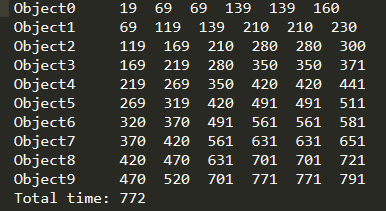
\includegraphics[scale=0.9]{pr.png}
            \caption{Результаты тестирования алгоритмов.}
            \label{png:testing:result}
        \end{figure}
\newpage